% !TEX root=../master.tex

\chapter{Introduction}
\label{chp:introduction}

\section{Problem Statement}
As multirotor unmanned aerial vehicles (UAVs) have become popular
platforms for commercial and consumer products over the past decade, a variety
of new use cases have emerged that require autonomous operation from larger
vehicles acting as moving, mobile base stations.
Such applications include
maritime surveillance, package delivery, and convoy
support (see~\figref{fig:drone_convoy_support}).
% State-of-the-art autonomous vehicle systems require robust solutions to three
% main problems: state estimation, motion planning, and control. In this thesis,
% we propose solutions to two of those three problems, state estimation and
% control, for a multirotor UAV landing on a moving vehicle.
% We leave the problem
% of motion planning as future work, providing some suggested direction
% in~\secref{sec:future_work}.
While there are
many facets to operating from moving vehicles, this thesis works toward creating
a robust solution to autonomously landing multirotor UAVs onto moving vehicles
in challenging conditions.

\begin{figure}[h]
  \centering
  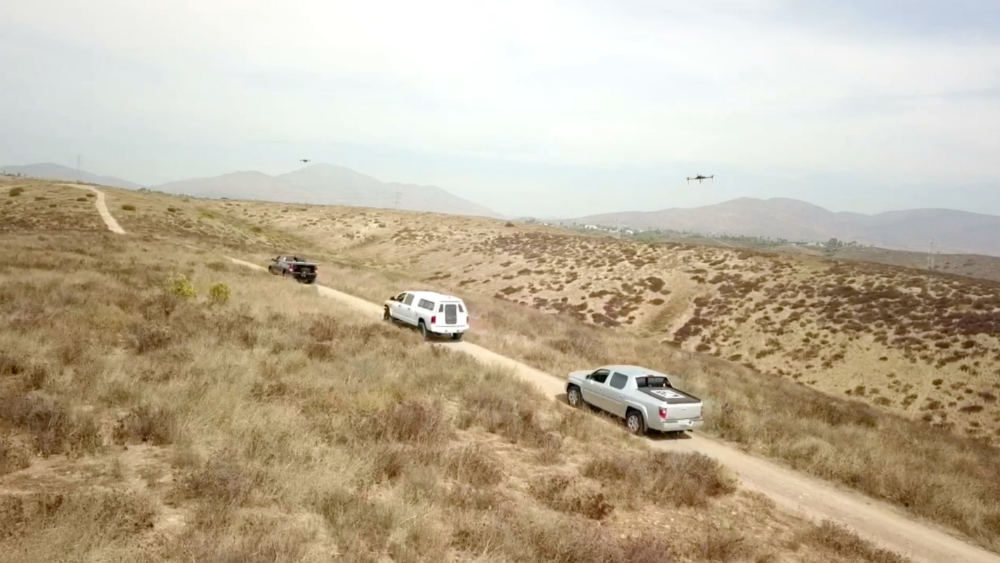
\includegraphics[width=4.5in]{figures/drone_convoy_support.png}
  \caption[UAV Convoy Support]{Multirotor UAVs used to increase
  situational awareness for a convoy of
vehicles.

Source:~\cite{ground_vehicle_drone}}
%
  \label{fig:drone_convoy_support}
\end{figure}


\section{Background}

Autonomous landing of multirotor UAVs onto moving vehicles has been previously
demonstrated in a variety of scenarios~\cite{wynn2019visual}; however, many problems still remain to
create a truly robust solution. Here we detail several of these outstanding
problems as they relate to the three principal problems that must be solved by
all autonomous UAVs: state estimation, motion planning, and control.

\subsection{State Estimation}
Most autonomous landing solutions require that the landing target vehicle is equipped
with a visual fiducial marker (i.e. see~\figref{fig:aruco_tag})
% Most landing methods assume that the target landing vehicle is equipped with a
% fiducial marker,
% such as the one shown in~\figref{fig:aruco_tag},
which serves as
the designated landing platform for the UAV.
In these methods, a camera mounted to the UAV detects the fiducial landing marker, providing
information about the relative pose of the target
vehicle~\cite{borowczyk2017autonomous}. These measurements are often used in a
filtering framework, such as a Kalman filter~\cite{kalman}, to produce a
% continuous
high-rate estimate of the relative state between the UAV and the target
vehicle. During landing, it is likely
that the fiducial marker is not detected for periods of time due to occlusion,
sun glare, or UAV motion. For this reason, it is important that the relative
motion between the target vehicle and the UAV is modeled and used to predict
the relative state when the fiducial marker is not detected.
However, even with a good model,
these methods quickly fail when the fiducial landing
marker is not detected for several seconds~\cite{ling2014precision}.

\begin{figure}[h]
  \centering
  
\includegraphics[width=2.5in]{figures/aruco_104.png}
  \caption[Visual Fiducial Landing Marker]{Visual fiducial markers such as this
    ArUco tag~\cite{garrido2016generation} are commonly used to assist in the
  landing of multirotor UAVs onto moving vehicles.}
  \label{fig:aruco_tag}
\end{figure}

When landing in challenging conditions such as strong winds, bright sun, or
dense fog, it is common that the fiducial marker may be undetected by the UAV
for long periods of time.
Therefore, to create a truly robust landing solution, an accurate estimate of
the state of the target vehicle must be maintained when the fiducial marker is
not detected for significant durations.
% the state estimation solution must maintain an accurate estimate of the relative
% state between the UAV and the target vehicle when the fiducial landing marker
% is not detected for significant durations.
Chapter~\ref{chp:estimation_paper}
describes an estimation algorithm, based on the error-state Kalman
filter~\cite{roumeliotis1999circumventing}, that tracks and estimates the locations of
visual features on the landing target vehicle to achieve this goal.

Visual feature
tracking and estimation is a common technique in the field of visual
odometry~\cite{qin2018vins}; however, almost all implementations assume the
tracked visual features are static with respect to an inertial reference frame.
In the landing scenario, the target vehicle occupies progressively more of the
field of view of the UAV's camera as the UAV descends. This makes it progressively
more difficult for typical visual odometry algorithms to track features,
resulting in a decreased
reliability of the estimates as the UAV approaches the landing target.
We also note that in most
applications, more precise state estimates are required as the UAV
approaches
the landing target to avoid obstacles and to ensure a gentle landing.
For these reasons, the described estimation algorithm
only tracks and estimates visual features that are rigidly attached to the
target vehicle.
Simulation and hardware tests of the proposed algorithm demonstrated accurate and consistent estimates
even when the fiducial marker was undetected
for long periods of time.

\subsection{Motion Planning}
The motion planning problem associated with autonomous vehicles is especially
important when 
% the path of the vehicle's motion is critical.
% This is commonly the case when
navigating close to obstacles. In the case of landing on moving vehicles, it is
often desired that the UAV descends vertically onto the landing pad to avoid
potential obstacles such as buildings, terrain, or vehicle superstructure.
When landing on certain vehicles, such as a boat at sea, the specific time of
touchdown may also be important to minimize the risk of damage to the UAV.

% Much work has been previously presented in the field of motion planning for
% small multirotor UAVs~\cite{mellinger2011minimum}.
Specific methods have been previously
presented to generate dynamically feasible trajectories for UAVs landing on moving
vehicles. One such method uses real-time model-predictive control techniques to
generate trajectories for a UAV landing on a moving car~\cite{baca2019autonomous}.
% It is likely that one or more of these solutions may be sufficient to create a
% robust landing system.
While improvements to these methods are not presented in this thesis, 
directions for future work related to motion planning are described
in~\secref{sec:future_motion_planning}.

\subsection{Control}
% A wide variety of control schemes for multirotor UAVs have been presented over
% the past two decades.
% A controller to robustly land a UAV onto a moving vehicle should be able to
% accurately track a time-dependent trajectory as described in the previous section.
% There are many control algorithms that sat
Many control algorithms have previously been presented that satisfy the
requirements for robust landing on moving vehicles.
% While many previously presented control algorithms may satisfy the
% requirements for robust landing on moving vehicles,
However, a recent
movement in the robotics community aims to appropriately deal with the evolution of a
robot's state along a manifold using Lie theory~\cite{sola2018micro}. Though
Lie theory has been widely applied to the field of state
estimation~\cite{sola2017quaternion, koch2017relative}, there is little 
work applying Lie theory to optimal control.

Chapter~\ref{chp:control_paper} derives a
linear-quadratic regulator (LQR) using Lie theory that computes control based on
the error-state dynamics of the system. Not only is this a more principled
approach than previous LQR methods, but it also achieves significant gains in computational efficiency.
Simulation and hardware results show that the derived controller can accurately
track a time-dependent trajectory, making it a good candidate for use in a
robust landing system.

\section{Summary of Contributions}
The research described in this thesis makes two significant contributions:
\begin{itemize}
\item A method of state estimation is developed that allows a multirotor UAV to
  continue to operate reliably with respect to a landing target vehicle even when a
  fiducial landing marker is not detected for significant periods of time.
% \item A method of state estimation is developed that maintains accurate and
  % consistent estimates of the state of a landing vehicle even when a fiducial landing
  % marker is not detected for significant periods of time by a multirotor UAV.
\item An optimal control scheme for a multirotor UAV is derived using an error-state,
  LQR formulation that enables accurate tracking of any dynamically feasible,
  time-dependent trajectory.
% \item An optimal control scheme for a multirotor UAV is derived in an error-state, linear
  % quadratic regulator (LQR) formulation. This provides an optimal control scheme
  % for a multirotor to follow any dynamically feasible, time-dependent
  % trajectory.
\end{itemize}

These contributions are demonstrated in both simulation and hardware
experiments found in Chapters~\ref{chp:estimation_paper}
and~\ref{chp:control_paper}. These results 
give us reason to believe that a
% show that a
complete and robust landing solution can be created by combining the proposed
state estimation and control schemes with a competent motion planner.

\section{Thesis Outline}

% The remainder of this thesis is organized as follows.
Chapter~\ref{chp:experimental_apparatus} details the hardware and software
systems used
in the experiments described in this thesis.
Chapter~\ref{chp:estimation_paper}
describes an improved method of state estimation for a multirotor UAV landing on
a moving vehicle.
% including results from simulation and hardware experiments.
% describes a state
% estimation algorithm that maintains accurate and consistent estimates even when
% a fiducial landing marker is not detected for significant periods of time.
Chapter~\ref{chp:control_paper} derives and demonstrates the performance of
an error-state LQR controller for a
multirotor UAV following a dynamically feasible, time-dependent trajectory.
Chapter~\ref{chp:conclusion} provides concluding remarks including
suggestions for future work that builds upon the work described in this
thesis.
